\chapter{Intégration sur $R^n$}

\setlength{\parindent}{0pt}
\renewcommand{\labelitemi}{\textbullet} % Utiliser des points noirs (•)

% ==================================================================================================================================
% 

\section{Tribu Produit}

Soit $(X_1,\mathcal{B}_1)$ et $(X_1,\mathcal{B}_2)$ deux espaces mesurables. 

\begin{definition}[Tribu Produit]
    La tribu produit sur $X_1 \times X_2$ est la plus petite tribu sur $X_1 \times X_2$ qui contient toutes les 
    parties du type $A_1 \times A_2$ où $A_1 \in \mathcal{B}_1$ et $A_2 \in \mathcal{B}_2$. \\
    On la note $ \mathcal{B} := \mathcal{B}_1 \otimes \mathcal{B}_2$. 
\end{definition}

\begin{prop}
    Soit $f : X \longleftrightarrow X_1 \times x_2, x \longmapsto (f_1(x),f_2(x))$ où $X$ est un espace mesurable. \\
    Alors f est mesurable sur $X$ ssi $f_1$ et $f_2$ sont mesurables sur $X$. 
\end{prop}

\begin{theorem}[Produit de tribu]
    Soit $n \in \N$, on a :
    \[ \mathcal{B}_{\R^2} = \mathcal{B}_\R \otimes \mathcal{B}_\R \quad \text{ et } \quad \mathcal{B}_{\R^n} = \bigotimes_{i=1}^n \mathcal{B} \] 
\end{theorem}

\begin{corollary}[Produit d'un borélien]
    Le produit d'un borélien est un borélien. 
\end{corollary}

\section{Mesure Produit}

Soit $(X_1,\mathcal{B}_1,\mu_1)$ et $(X_1,\mathcal{B}_2,\mu_2)$ deux espaces mesurés. 

\begin{definition}[Mesure Produit]
    Il existe une mesure $\mu$ sur $(X_1 \times X_2, \mathcal{B}_1 \times \mathcal{B}_2)$ telle que 
    $ \forall A_1 \in \mathcal{B}_1, \forall A_2 \in \mathcal{B}_2$, on ait :
        \[ \mu (A_1 \times A_2) = \mu_1(A_1) \times \mu_2(A_2) \]
    elle est appelée mesure produit sur $X_1 \times X_2$ et notée $\mu_1 \otimes \mu_2$. 
\end{definition}

\newpage 

\begin{definition}[Espace mesuré produit]
    Soit $ B \in \mathcal{B}_1 \times \mathcal{B}_2$, on a :
        \[ \mu(B) = \inf \sum_{n=0}^{\infty} \mu (B_n) \] 
    où $(B_n)_{n \in \N}$ est la suite de l'ensemble des recouvrements dénombrables de $B$ par des produits cartésiens. \\
    $(X_1 \times X_2,\mathcal{B}_1 \otimes \mathcal{B}_2,\mu_1 \otimes \mu_2)$ est donc appelée espace mesuré produit. 
\end{definition}

\section{Intégration sur $\R^n$}

\begin{theorem}[Fubini-Tonelli]
    \begin{enumerate}
        \item \underline{Tonelli :} Soit $F \in \overline{\mathcal{M}_+}(X)$ telle que :
            \[ f :
                \begin{cases}
                    X_1 \times X_2 \longrightarrow \overline{\R_+} \\ 
                    (x_1,x_2) \longmapsto f(x_1,x_2)
                \end{cases} \] 
            Alors :
                \begin{align*}
                    \int_{X_1 \times X_2} f \; d \mu    &= \int_{X_1} \Bigl( \int_{X_2} f(x_1,.) \; d \mu_2 \Bigr) \; d \mu_1(x_1) \\
                                                        &= \int_{X_2} \Bigl( \int_{X_1} f(.,x_2) \; d \mu_1 \Bigr) \; d \mu_2(x_2)
                \end{align*}
        \item \underline{Fubini :} Soit $f \in \mathcal{L}^1(X_1 \times X_2)$. Alors la formule précédente est vraie 
                \begin{align*}
                    \int_{X_1 \times X_2} f \; d \mu    &= \int_{X_1} \Bigl( \int_{X_2} f(x_1,.) \; d \mu_2 \Bigr) \; d \mu_1(x_1) \\
                                                        &= \int_{X_2} \Bigl( \int_{X_1} f(.,x_2) \; d \mu_1 \Bigr) \; d \mu_2(x_2)
                \end{align*}
                \underline{ici} $f(.,x_2)$ est intégrable sur $X_1$ pour presque tout $x_2 \in X_2$ donc $\int f \; d \mu_1$ est bien définie p.p sur $X_2$
    \end{enumerate}
\end{theorem}

\begin{definition}[Matrice Jacobienne]
    Soit $ \phi : U \rightarrow V$ où $U$ est un ouvert de $R^k$ et $V$ un ouvert de $\R^n$. La matrice Jacobiennne de $\phi$ est la fonction :
        \[ D_\phi :
            \begin{cases}
                U \longrightarrow \mathcal{M}_{n,k}(\R) \\
                x \longmapsto \Bigl( \frac{\partial \phi ^i}{\partial x_j} \Bigr) _{1 \leq i,j \leq k,n}
            \end{cases} \] 
    Le jacobien de $\phi$ est la fonction :
        \[ J_\phi :
            \begin{cases}
                U \longrightarrow \R_+ \\ 
                x \longmapsto \sqrt{\det (^t D_\phi \times D_\phi)}
            \end{cases}
        \]
        car $^t D_\phi \times D_\phi \in \mathcal{M}_{k,k}(\R)$.
    \begin{itemize}
        \item \underline{si $k = n$ :} $ \boxed{J_\phi(x) = | \det D_\phi |} $
        \item \underline{si $ k =1$ :} $ J_\phi(x) = \sqrt{\sum_{i=1}^{n} \phi^{i}(x)} = \| \phi'(x) \|$  
    \end{itemize}
\end{definition}

\begin{definition}[$C^p$-difféomorphisme]
    Supposons que $k=n$, $\phi$ est un $C^p$-difféomorphisme si 
    \[ \phi : U \longrightarrow V \]
    où $U$ et $V$ sont deux ouverts de $\R^n$ et, de plus :
    \begin{enumerate}
        \item $\phi \in C^p(U)$ 
        \item $\phi$ est bijective de réciproque $\phi^{-1}$
        \item $\phi^{-1} \in C^p(U)$ 
    \end{enumerate}
\end{definition}

\begin{theorem}[Inversion Globale]
    Soit $\Psi : U \subset \R^n \longrightarrow V \subset \R^n$ tel que $\Psi \in C^p$ et $\Psi$ injective. 
    \begin{itemize}
        \item[\underline{si}] $ \forall x \in U, D_{\Psi_x}$ est inversible
        \item[\underline{alors}]  $\Psi : U \longrightarrow \Psi(V)$ est un $C^p$-difféomorphisme et $\Psi(U)$ est un ouvert de $\R^n$
    \end{itemize}
\end{theorem}

\begin{theorem}[Changement de variable]
    Soient $U,V \subset \R^n$ deux ouverts et $\Psi : U \longrightarrow V$ un $C^p$-difféomorphisme. 

    \vspace{0.5cm}
    \begin{minipage}{0.45\textwidth}
        \[
        \begin{tikzcd}[scale=1.25\textwidth]
            U \arrow[r, "\Psi"] \arrow[rd, "\int f \circ \Psi" swap] & V \arrow[d, "\int f"] \\
                                                                   & \mathbb{R}_+ \text{ ou } \mathbb{C}
        \end{tikzcd}
        \]
        \[ \text{où } f : V \longrightarrow \overline{R_+} \text{ où } \C \]
    \end{minipage}
    \hfill
    \begin{minipage}{0.45\textwidth}
        \emph{Autrement dit, $\Psi$ donne les anciennes variables en fonction des nouvelles. 
        Le raisonnement est similaires aux matrices de passage.}
    \end{minipage}
    \vspace{0.5cm}
    \begin{itemize}
        \item[\underline{si}] $f \in \overline{\mathcal{M}_+}(V)$ \underline{alors} :
            \[ \boxed{ \int_V f \; d \lambda_n = \int_U f \circ \Psi \times J_\phi \; d \lambda_n} \] 
        \item[\underline{si}] $f \in {\mathcal{M}}(V)$ on a : $ f \in \mathcal{L}^1(U) \Longleftrightarrow (f \circ \Psi) \times J_\phi \in \mathcal{L}^1(U) $
             et dans ce cas :
                \[ \int_V f \; d \lambda_n = \int_U (f \circ \Psi) \times J_\phi \; d \lambda_n \]
    \end{itemize}
\end{theorem}


\begin{example}[Changement de variable polaire]
    Soient $(r,\theta) \in \R_+^* \times ]0,2\pi[$ tels que $ \Psi(r,\theta) = (r \cos \theta, r \sin \theta)$ 

    \begin{minipage}{0.45\textwidth}
        \begin{center}
        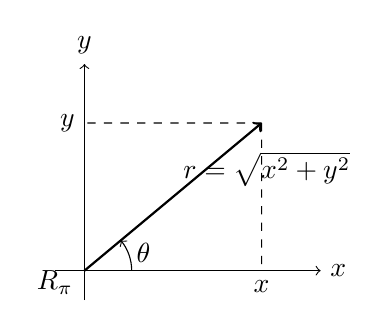
\begin{tikzpicture}[scale=0.75]
            % Axes
            \draw[->] (-0.5,0) -- (4,0) node[right] {$x$};
            \draw[->] (0,-0.5) -- (0,3.5) node[above] {$y$};
            
            % Labels for R^2 and R_+
            \node at (-0.5, -0.2) {$\mathbb{R}_\pi$};
            
            % Point and vector r
            \coordinate (O) at (0,0);
            \coordinate (P) at (3,2.5);
            \draw[->, thick] (O) -- (P) node[midway, above right] {$r = \sqrt{x^2 + y^2}$};
            
            % Dotted lines to the axes
            \draw[dashed] (P) -- (3,0) node[below] {$x$};
            \draw[dashed] (P) -- (0,2.5) node[left] {$y$};
            
            % Angle theta
            \draw[->] (0.8,0) arc[start angle=0,end angle=40,radius=0.8];
            \node at (1,0.3) {$\theta$};
        \end{tikzpicture}
        \end{center}
    \end{minipage}
    \hfill 
    \begin{minipage}{0.45\textwidth}
        \[ \Psi : 
            \begin{cases}
                \R_+^* \times ]0,2\pi[ \rightarrow \R^2 \backslash \R_\pi \\ 
                (r,\theta) \longmapsto (x,y) = (r \cos \theta,r \sin \theta) 
            \end{cases}
        \]
    \end{minipage}

    Alors : 
        \[ J_{\Psi(r,\theta)} =
            \begin{pmatrix}
                \cos \theta & - r \sin \theta \\ 
                \sin \theta & r \cos \theta 
            \end{pmatrix}
        \text{et } |J_{\Psi(r,\theta)}| = r \cos^2 \theta + r \sin^2 \theta = r \in \R_+^* \] 
\end{example}

\newpage
\begin{corollary}[Passage en polaire]
    Soit $\Psi$ le passage en coordonnées polaires. Alors $\Phi$ est un $C^\infty$-difféomorphisme et 
    pour tout $f \in \overleftarrow{\mathcal{M}_+}(\R^2)$, on a :
        \[  \int_U f(x,y) \;d \lambda_2 = \int_V f(r \cos \theta, r \sin \theta) \times r \; dr d \theta \]
    où $V = \R_+^* \times ]0,2\pi[$
\end{corollary}

\begin{example}[Aire d'un disque]

    Aire d'un disque avec le corollaire fraîchement énoncé :

    \begin{minipage}{0.45\textwidth}
        Soit $A$ l'aire du disque de rayon $R$ centré en $(0,0)$.
        Alors
            \begin{align*}
                A &= \lambda_2(Disque) \\
                &= \int_{\R^2} 1_{Disque}(x,y) \; dxdy
            \end{align*}
    \end{minipage}
    \hfill 
    \begin{minipage}{0.45\textwidth}
        \begin{center}
        \begin{tikzpicture}[scale=0.75]
            % Axes
            \draw[->] (-3,0) -- (3,0) node[right] {$x$};
            \draw[->] (0,-3) -- (0,3) node[above] {$y$};
            
            % Filled Disk
            \filldraw[pattern=north east lines, pattern color=black, draw=black] (0,0) circle (2); % Change 2 to the desired radius
        
            % Label for radius
            \node at (2.5,-0.5) {$r$};
            
            % Center label
            % \node at (0.2, -0.2) {$O$};
        \end{tikzpicture}
        \end{center}
    \end{minipage}
    \begin{align*}
        &= \int_{\R_+^* \times ]0,2\pi[} 1_{Disque}(r \cos \theta, r \sin \theta) \times r \; dr d \theta \\
        &= \int_{0}^{\infty} \Biggl( \int_{0}^{2\pi} 1_{[0,\R[}(r) \times r \; d \theta \Biggr) \; dr \\
        &= \Biggl( \int_{0}^{\infty} 1_{[0,\R[}(r) \times r \; d r \Biggr) \times 2 \pi \\
        &= 2 \pi \int_{0}^{R} r \; dr = 2 \pi \frac{R^2}{2} = \pi R^2 
    \end{align*}
\end{example}

\begin{example}[Gaussienne sur $\R$]
    Soit $\gamma$ la gaussienne sur $\R$ telle que $ \gamma = \int_\R e^{-x^2} \; dx = \sqrt{\pi}$. 
    Vérifions ce résultat. 

    \begin{minipage}{0.45\textwidth}
        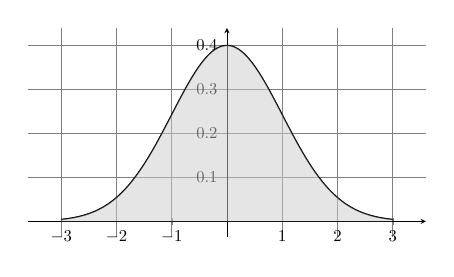
\begin{tikzpicture}[scale=0.6]
            \begin{axis}[
                axis lines = middle,
                grid = both,                 % Fond quadrillé
                grid style={line width=0.5pt, draw=black!50}, % Style des lignes du quadrillage
                xlabel = {},
                ylabel = {},
                domain = -3:3,
                samples = 100,
                width=10cm,
                height=6cm,
                xtick distance=1,            % Distance entre les graduations sur l'axe des x
                ytick distance=0.1,          % Distance entre les graduations sur l'axe des y
                axis line style={black},     % Couleur des axes
                enlarge x limits=0.1,        % Dépassement des axes sur l'axe des x
                enlarge y limits=0.1,        % Dépassement des axes sur l'axe des y
                ]
            \addplot[
                black,                      % Courbe en noir
                thick                       % Épaisseur de la courbe
            ] {exp(-x^2 / 2) / sqrt(2*pi)};
            
            % Dessiner la zone sous la courbe avec un fond gris clair
            \addplot [
                domain=-3:3,
                samples=100,
                fill=black!20,              % Remplissage gris clair
                opacity=0.5,                % Opacité du remplissage
                ] {exp(-x^2 / 2) / sqrt(2*pi)} \closedcycle;
            \end{axis}
        \end{tikzpicture}
    \end{minipage}
    \hfill 
    \begin{minipage}{0.45\textwidth}
        \begin{align*}
            \gamma &= \Biggl( \int_\R e^{-x^2} \; dx \Biggr) \Biggl( \int_\R e^{-y^2} \; dy \Biggr) \\
                    &= \int_\R \Biggl( \int_\R e^{-y^2} \; dy \Biggr) e^{-x^2} \; dx \\
                    &= \int_\R \int_R e^{-x^2-y^2} \; dxdy 
        \end{align*}
    \end{minipage}
    
    \vspace{0.5cm}
    D'après le théorème de Tonelli :
    \[ \int_\R \int_R e^{-x^2-y^2} \; dxdy  = \int_{R^2 \times \R^2} e^{-x^2-y^2} \; dxdy  \] 
    D'après le changement de variable polaire :
    \[ \forall (x,y) \in \R^2 \backslash R_\pi, \quad \exists (x,\theta) \in \R_+^* \times ]0,2\pi[ \text{ tq} \quad (x,y) = (r \cos \theta, r \sin \theta) \]
    D'où : 
    \begin{align*}
        \dots &= \int_{0}^{2\pi} \int_{0}^{\infty} r e^{-r^2 \cos^2 \theta - r^2 \sin^2 \theta} \; dr d\theta \\
            &= \int_{0}^{2\pi} \int_{0}^{\infty} r e^{-r^2} \; dr d \theta = \int_{0}^{2\pi} \Bigl[ - \frac{e^{-r^2}}{2}\Bigr]_0^\infty \; d \theta \\
            &= \int_{0}^{2\pi} \frac{1}{2} \; d \theta = \Bigl[ \frac{1}{2} \theta\Bigr]_0^{2\pi} = \pi 
    \end{align*}
    donc $ \gamma^2 = \pi \Longleftrightarrow \gamma = \pi $
\end{example}

\begin{theorem}[Changement de variable spérique]
    
    \begin{minipage}{0.45\textwidth}
        \[ \Psi :
        \begin{cases}
            \R_+ \times ]-\pi, \pi[ \times ]0,\pi[ \longrightarrow \R^3 \backslash P \\
            (r,\theta,\varphi) \longmapsto     \begin{pmatrix}
                                                x \\
                                                y \\
                                                z 
                                            \end{pmatrix}
            = 
            \begin{pmatrix}
                r \sin \varphi \cos \theta \\
                r \sin \varphi \sin \theta \\
                r \cos \theta
            \end{pmatrix}
        \end{cases}
    \] 
    \begin{align*}
        x &= p \cos \theta = r \sin \varphi \cos \theta \\
        y &= p \sin \theta = r \sin \varphi \sin \theta \\
        z &= r \cos \theta
    \end{align*}
    \end{minipage}
    \hfill 
    \begin{minipage}{0.45\textwidth}
        \begin{center}
            \begin{tikzpicture}[scale=1.25]
                % Points
                \coordinate (origine) at (0,0,0);
                \coordinate (axeX) at (3,0,0);
                \coordinate (axeY) at (0,3,0);
                \coordinate (axeZ) at (0,0,3);
                \coordinate (vecteur) at (2.5,2,2);
    
                % Projections
                \coordinate (projY) at (0,2.5,0);
                \coordinate (projX) at (2.2,0,0);
                \coordinate (projZ) at (0,0,2.7);
                \coordinate (projPlan) at (2.7,0,2.7);
    
                % Dessin des axes
                \draw[->] (origine) -- (axeX) node[right] {$y$};
                \draw[->] (origine) -- (axeY) node[right] {$z$};
                \draw[->] (origine) -- (axeZ) node[right] {$x$};
    
                % Dessin du vecteur
                \draw[->, thick] (origine) -- (vecteur) node[right] {$(x,y,z)$};
    
                % Dessin du vecteur projeté
                \draw[->] (origine) -- (projPlan) node[right] {$p = r \sin \varphi$}; 
    
                % Dessins des projections
                \draw[dotted] (vecteur) -- (projY);
                \draw[dotted] (vecteur) -- (projPlan);
                \draw[dotted] (projPlan) -- (projZ);
                \draw[dotted] (projPlan) -- (projX);
    
                % Dessin des points
                \filldraw (projX) circle (0.5pt);
                \filldraw (projY) circle (0.5pt);
                \filldraw (projZ) circle (0.5pt);
                \filldraw (projPlan) circle (0.5pt);
    
                % Tracer l'angle entre les deux vecteurs
                \draw pic[draw, fill=gray!30, angle radius=1cm, "$\varphi$"] {angle=vecteur--origine--axeY};
                \draw pic[draw, fill=gray!30, angle radius=1cm, "$\theta$"] {angle=axeZ--origine--projPlan};
            \end{tikzpicture}
        \end{center}
    \end{minipage}

    \vspace{0.5cm}

    $\Psi$ est un $C^\infty$-difféomorphisme de Jacobien :
    \[ J_\Psi
        \begin{vmatrix}
            \sin \varphi \cos \theta & - r \sin \varphi \sin \Theta & r \sin \theta \cos \theta \\
            \sin \theta & r \sin \varphi \cos \theta & r \sin \varphi \cos \theta \\
            \cos \theta & 0 & - r \sin \varphi
        \end{vmatrix}
        \dots = r^2 \sin \theta > 0 
    \]
    
\end{theorem}